\chapter{Introduction}
\label{ch:Introduction}
\pagenumbering{arabic} \setcounter{page}{1}

Named Entity Recognition (NER) is a foundational task in natural language processing (NLP), concerned with identifying and classifying entities such as persons, organizations, and locations in unstructured text. This technical report outlines the development of a custom NER solution designed to process news articles and extract these entity types accurately under constrained evaluation criteria. The project was completed as part of a time-bound applied machine learning assessment, with requirements that span both model performance and deployment readiness.

\section{Background}

Many off-the-shelf NLP models offer generic entity recognition capabilities. However, such models often fail to meet specific evaluation conditions — such as exact multi-word matches or fine-grained disambiguation of organizational names. Furthermore, real-world applications demand solutions that are not only accurate, but also reproducible, deployable, and performant under load.

This project was designed to demonstrate competency in end-to-end ML system development: from initial data exploration and preprocessing, through model design and training, to deployment as a REST API and evaluation under concurrent usage scenarios. The dataset used in this task consists of news articles with annotated entities across the three categories of interest.

\section{About this Report}

This technical report documents the approach, decisions, and results of the NER system development. It covers the complete project lifecycle — including data analysis, baseline testing, model experimentation, deployment via Docker, and performance validation using Locust.

The deliverables included:
\begin{itemize}
  \item An ML pipeline that improves upon baseline NER performance
  \item A reproducible training setup with tracked experiments
  \item A REST API that takes a CSV as input and returns predictions in a specific format
  \item A Dockerized deployment for seamless execution
  \item Load testing results demonstrating support for 20+ concurrent users
\end{itemize}

\section{Chapter List}

\textbf{Chapter \ref{ch:Introduction}} Explains the task that is solved with this solution.

\textbf{Chapter \ref{ch:Data-Exploration}} Describes and discusses dataset

\textbf{Chapter \ref{ch:Data-Preparation}} Every step to modify the dataset into a more usable dataset

\textbf{Chapter \ref{ch:Software-Architecture}} General software design as uml diagram.

\textbf{Chapter \ref{ch:Model-Selection}} A listing of all the models implemented and tested.


\textbf{Chapter \ref{ch:Evaluation}} Evaluation \& Testing. Summarizes model performance, benchmarking results, and system behaviour under concurrent load.




\textbf{Chapter \ref{ch:Conclusion}} Conclusion. Highlights key findings and suggests directions for future improvement.

% \textbf{Chapter \ref{ch:usingLatex}} Using \LaTeX. \textcolor{red}{COMMENT OUT THIS SECTION IN FINAL VERSION.}

\section{Conclusion}

This introduction set the stage for the technical report by describing the problem, summarizing the goals and deliverables, and outlining the structure of the document. The following chapters provide detailed insights into each stage of the project.


\chapter{Data-Exploration}
\label{ch:Data-Exploration}

\section{Entity Format Analysis}

A closer look at the entity label columns revealed the following:

\begin{itemize}
  \item \textbf{Persons and Organizations:}  
  These fields contain a semicolon-separated list of \texttt{entity,id} pairs. For example:
  \begin{verbatim}
  Joe Biden,135; Karen Jan Pierre,1533; Mohammed Ben Salman,55
  \end{verbatim}
  Each entry represents a full entity name and an associated numerical ID. The origin and purpose of these IDs remain unknown, and some entities appear multiple times with different IDs.

  \item \textbf{Locations:}  
  Unlike the other two columns, this field uses a \textbf{comma-separated} format for listing entity names:
  \begin{verbatim}
  White House, Yemeni, United States, Yemen, Saudi Arabia
  \end{verbatim}
  There are no associated IDs for location entities.
\end{itemize}

To better understand the structure and frequency of the labeled entities, all unique entities were extracted and saved to:
\begin{quote}
\texttt{misc/entities\_reversed\_dict.json}
\end{quote}
This allowed inspection of the vocabulary and confirmed that the numeric IDs are \textbf{not unique} and provide no reliable information for downstream processing.



\section{Conclusion}

The dataset is a structured collection of news article snippets with annotated named entities for persons, organizations, and locations. Textual patterns and references (e.g., frequent mentions of CNN and political topics) strongly suggest that the content was downloaded or scraped from a news website.

The entity fields are inconsistently formatted: \texttt{persons} and \texttt{organizations} include non-unique numeric IDs, while \texttt{locations} are comma-separated with no IDs. After analysis, it was concluded that the numeric IDs do not carry consistent meaning and will be removed. Furthermore, to ensure consistency across all entity types, each field will be normalized into a semicolon-separated list of clean entity names.

This exploration phase highlights the importance of harmonizing and sanitizing the dataset before modeling. The next step is to implement the data preparation pipeline based on these insights.


\chapter{Data Preparation}
\label{ch:Data-Preparation}

This chapter describes the cleaning and preprocessing steps applied to the dataset before training and evaluation. The goal was to standardize entity formats, clean noisy input text, and prepare suitable subsets for fine-tuning and testing. All transformations were implemented in the notebook \texttt{01\_data\_preparation.ipynb}.

\section{Cleaning Decisions}

Based on the insights from data exploration, the following harmonization and cleanup operations were carried out:

\begin{itemize}
  \item \textbf{Entity ID Removal:} The \texttt{persons} and \texttt{organizations} columns contained entries in the format \texttt{Entity Name,ID}, e.g., \texttt{Joe Biden,135}. Since the IDs were non-unique and their meaning was unclear, they were discarded. Only the clean entity names were retained.
  
  \item \textbf{Delimiter Normalization:} The \texttt{locations} column used a comma-separated format, whereas \texttt{persons} and \texttt{organizations} were semicolon-separated. To ensure consistency, all three fields were converted to use semicolons as the standard delimiter.
  
  \item \textbf{HTML and Structured Text Cleanup:} The \texttt{text} column contained both HTML fragments and prefixed strings like \texttt{"articleBody"}. Two cleaning strategies were applied:
    \begin{itemize}
      \item Text entries starting with \texttt{<html} were converted to markdown using the \texttt{markdownify} package with stripped anchor tags.
      \item Entries starting with \texttt{"articleBody"} were parsed by extracting the inner text between quotation marks.
    \end{itemize}
\end{itemize}

These steps ensured that the textual content and entity annotations were consistent, clean, and ready for downstream processing.

\section{Data Splitting}

To support modular experimentation, the cleaned dataset was split into two equally sized subsets using a reproducible split strategy:

\begin{itemize}
  \item \textbf{Total dataset size:} 692 rows
  \item \textbf{Split ratio:} 50/50
  \item \textbf{Random seed:} \texttt{random\_state=42}
\end{itemize}

The purpose of the split was to separate concerns between model fine-tuning and general evaluation:

\begin{itemize}
  \item \textbf{Fine-tuning Subset (346 rows):} This portion was used to fine-tune a custom NER model. It contains cleaned text and standardized entity fields and is saved as \texttt{full\_data\_clean\_finetune.csv}.
  
  \item \textbf{Evaluation Subset (346 rows):} The remaining half of the data was reserved for:
    \begin{itemize}
      \item Evaluation through the deployed REST API
      \item Testing out-of-the-box or zero-shot baseline models
      \item Prompt-based training or other auxiliary use cases
    \end{itemize}
    It is saved as \texttt{full\_data\_clean.csv}.
\end{itemize}

This strategy ensures that model performance is evaluated on a disjoint set of data, free from contamination by fine-tuning examples.

\section{Token Count Analysis}

To gain insight into the input length distribution, the number of tokens per article was calculated using the \texttt{tiktoken} tokenizer configured for the \texttt{gpt-4o} model. Token counts were added as a new column, and their distribution was visualized as a histogram.

The resulting histogram showed significant variance in document length, with some entries exceeding several hundred tokens. This variability was considered in later modeling stages to inform batching strategies and maximum sequence lengths.

\begin{figure}[h]
  \centering
  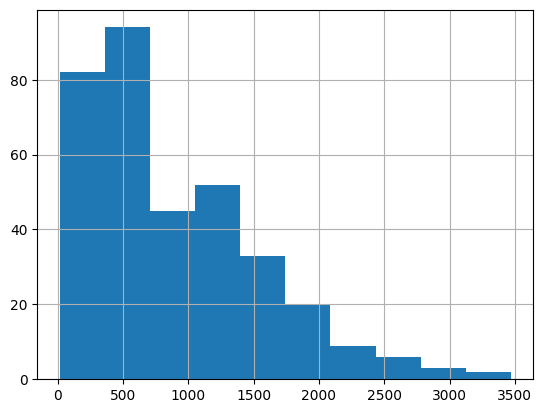
\includegraphics[width=0.65\textwidth]{imgs/token-hist.png}
  \caption{Histogram of token counts per article in the fine-tuning dataset}
  \label{fig:token-hist}
\end{figure}

\section{Exported Files}

The following files were created and exported during preprocessing:

\begin{itemize}
  \item \texttt{full\_data\_clean\_finetune.csv} – Cleaned subset used for model fine-tuning.
  \item \texttt{full\_data\_clean.csv} – Cleaned subset used for evaluation and deployment.
\end{itemize}

All files were stored in the project’s \texttt{FILES\_DIR} for reproducible reuse across the pipeline.

\section{Conclusion}

The dataset was successfully cleaned, harmonized, and split into subsets appropriate for both training and evaluation. Entity formats were standardized, noisy HTML and wrappers were removed, and token distributions were examined to guide modeling decisions. These steps ensure a clean and robust input foundation for the upcoming modeling phase.

\chapter{Software Architecture Design}
\label{ch:Software-Architecture}

This chapter describes the architecture of the NER system, with a strong emphasis on modularity, reproducibility, and extensibility. The system follows scikit-learn’s design philosophy, centered around \texttt{fit}, \texttt{predict}, and \texttt{transform} interfaces to ensure compatibility with established machine learning workflows.

\section{Architecture Design}

The core abstraction of the system is the \texttt{SingleEntityExtractor} class, which provides a reusable and extensible interface for implementing named entity extractors specific to a single entity type — namely \texttt{persons}, \texttt{organizations}, or \texttt{locations}.

\subsection{SingleEntityExtractor}

The \texttt{SingleEntityExtractor} class inherits from \texttt{sklearn.base.BaseEstimator} and defines a clean interface with the following core methods:

\begin{itemize}
  \item \textbf{\texttt{fit}} — Trains the model on a given text and entity label set.
  \item \textbf{\texttt{predict}} — Applies the model to extract entities from raw text.
  \item \textbf{\texttt{evaluate}} — Computes and logs evaluation metrics using both macro and micro averaging.
  \item \textbf{\texttt{fit\_predict}} — Utility wrapper for end-to-end training and inference.
\end{itemize}

It also tracks internal statistics such as processing time, sample size, word counts, and metric scores for \textbf{training}, \textbf{inference}, and \textbf{evaluation} phases.

Metrics are computed using macro- and micro-averaged precision, recall, F1, accuracy, and Jaccard similarity. The evaluation method distinguishes between:
\begin{itemize}
  \item \textbf{Strict multi-word matching} for \texttt{persons} and \texttt{locations}
  \item \textbf{Multi-word and partial-word matching} for \texttt{organizations}
\end{itemize}

Each model type (e.g., regex-based, transformer-based) inherits this base class and implements the abstract methods \texttt{\_fit} and \texttt{\_predict}, ensuring predictable behavior and consistency across extractors.

\subsection{MultiEntityExtractor}

The \texttt{MultiEntityExtractor} acts as a manager that aggregates multiple \texttt{SingleEntityExtractor} instances under one unified interface. Its responsibilities include:

\begin{itemize}
  \item Managing a dictionary of named entity extractors (e.g., \texttt{persons}, \texttt{organizations}, \texttt{locations}).
  \item Fitting and predicting with all sub-models in parallel.
  \item Returning a single DataFrame with one column per entity type.
\end{itemize}

This class supports methods like \texttt{add\_extractor}, \texttt{remove\_extractor}, and \texttt{get\_extractor} to encourage dynamic composition and flexibility. The predictions of individual extractors are post-processed to conform to the required semicolon-separated string output format.


\begin{figure}[h]
  \centering
  \includegraphics[width=0.65\textwidth]{imgs/uml.png}
  \caption{UML diagram shows the architecture of the extractor classes.}
  \label{fig:uml}
\end{figure}

\section{Design Rationale}

The architecture follows these core principles:

\begin{itemize}
  \item \textbf{Modularity:} Each entity type is handled independently, allowing plug-and-play flexibility for experimenting with different models or training objectives per entity class.
  \item \textbf{Reusability:} The abstract base class design allows future models to be integrated with minimal changes.
  \item \textbf{Composability:} The \texttt{MultiEntityExtractor} enables combining extractors in a structured and maintainable way.
  \item \textbf{Traceability:} Time and metric tracking are built into the base class for reproducible evaluation.
\end{itemize}

\section{Trade-offs}

While separating extractors by entity type provides maximum flexibility and encapsulation, it comes with a performance cost: the runtime is approximately tripled compared to a unified model. In practice, this trade-off is acceptable for offline inference and batch API calls, but could become a bottleneck under high-throughput real-time settings.

It is also possible to inherit directly from the \texttt{MultiEntityExtractor} and implement a joint model for all entity types. This was considered out of scope for the current project but remains a viable path for future optimization.

\section{Conclusion}

The system architecture is centered around clean, modular interfaces following the scikit-learn paradigm. This ensures clarity, extensibility, and consistency across the training, prediction, and evaluation pipeline. The separation between single-entity and multi-entity extractors enables a flexible yet powerful foundation for future experimentation and deployment.

\chapter{Model Selection}
\label{ch:Model-Selection}

This chapter outlines the various models implemented for the named entity recognition (NER) task. Each model targets the extraction of \texttt{persons}, \texttt{organizations}, or \texttt{locations}, and is evaluated independently. The best-performing model for each entity type is selected in Chapter~\ref{ch:Evaluation}.

\section{Overview}

A modular approach is adopted to allow flexibility in selecting the most appropriate model for each entity type. This enables mixing lightweight, high-speed methods with more accurate but heavier alternatives, depending on the use case.

\section{Selected Models}

\subsection{Naive Sliding Window Extractor}

The \texttt{SlidingWindowExtractor} is a simple rule-based model designed as a baseline. It inherits from the \texttt{SingleEntityExtractor} base class and implements a brute-force matching strategy.

\textbf{Implementation Details:}

During the \texttt{fit} phase, the extractor flattens the entity labels into a dictionary where each key is the full entity string and the value is its tokenized form. This list serves as the reference vocabulary during inference.

In the \texttt{predict} phase, the model performs the following steps:

\begin{enumerate}
  \item Cleans the input text using a regular expression that removes all non-alphanumeric characters.
  \item Tokenizes the cleaned input text.
  \item Iterates through the text using a fixed-size sliding window for each entity in the training vocabulary.
  \item Matches the window content with each entity’s token sequence.
  \item Appends any full matches to the prediction output.
\end{enumerate}

All results are returned as lists of semicolon-joinable entity strings, in line with the system’s output format conventions.

\textbf{Advantages:}
\begin{itemize}
  \item Simple and interpretable logic.
  \item No dependencies on external NLP libraries.
  \item Deterministic behavior and fast training time.
\end{itemize}

\textbf{Drawbacks:}
\begin{itemize}
  \item Poor generalization to unseen entities.
  \item High time complexity during inference due to exhaustive window scanning.
  \item Vulnerable to tokenization mismatches, casing, and punctuation variance.
\end{itemize}

While not suitable for production use, the sliding window extractor is useful as a diagnostic tool and sanity check for verifying entity format and coverage.


\subsection{spaCy NER Extractor}

The \texttt{SpacyEntityExtractor} leverages spaCy’s built-in named entity recognition pipeline as a lightweight, pretrained solution. It wraps around \texttt{en\_core\_web\_sm}, a fast English model designed for general-purpose NLP.

\textbf{Implementation Details:}

The extractor inherits from \texttt{SingleEntityExtractor} and uses spaCy’s \texttt{Doc.ents} to extract entities of interest. A label mapping is used to align the task-specific categories to spaCy’s internal label scheme:

\begin{itemize}
  \item \texttt{persons} → \texttt{["PERSON"]}
  \item \texttt{organizations} → \texttt{["ORG"]}
  \item \texttt{locations} → \texttt{["LOC", "GPE"]}
\end{itemize}

The model is fully pretrained and requires no fitting. During prediction, each input text is processed by the spaCy pipeline, and relevant entities are filtered using the mapped labels. An optional flag \texttt{require\_full\_name} excludes single-word entities when set to \texttt{True}, which is useful for enforcing stricter multi-token match evaluation (e.g., \texttt{"Joe Biden"} but not \texttt{"Biden"}).

The model loading logic includes a fallback mechanism: if the model is not available locally, it is downloaded on the fly using \texttt{spacy.cli.download()}.

\textbf{Advantages:}
\begin{itemize}
  \item Lightweight and fast, even on CPU.
  \item Pretrained and ready to use without additional training.
  \item Handles sentence segmentation, tokenization, and entity recognition end-to-end.
\end{itemize}

\textbf{Drawbacks:}
\begin{itemize}
  \item Limited performance on domain-specific or rare entities.
  \item Label space is fixed; adaptation requires training a custom spaCy pipeline.
  \item No explicit support for entity linking or disambiguation.
\end{itemize}

Overall, the \texttt{SpacyEntityExtractor} serves as a strong zero-configuration baseline, ideal for benchmarking and rapid prototyping.


\subsection{Zero-Shot LLM Extractor (LangChain + GPT)}

The \texttt{LangChainEntityExtractor} implements a zero-shot named entity recognition model using the \texttt{gpt-4o-mini} API via the LangChain framework. This approach uses prompting and structured output parsing to extract full-name entities without explicit training.

\textbf{Implementation Details:}

This extractor inherits from \texttt{SingleEntityExtractor} and leverages the LangChain abstraction to compose prompts, send them to the LLM, and parse structured responses into a Pydantic model.

Key components include:

\begin{itemize}
  \item \textbf{Model:} \texttt{gpt-4o-mini} (via \texttt{ChatOpenAI}) with zero temperature for deterministic output.
  \item \textbf{Output Schema:} The model must return an instance of \texttt{LLMResult}, a Pydantic object with optional lists of typed entities: \texttt{persons}, \texttt{organizations}, and \texttt{locations}.
  \item \textbf{Prompt Template:} Composed using a \texttt{ChatPromptTemplate} with:
    \begin{itemize}
      \item Format instructions generated from the Pydantic parser.
      \item Optional examples constructed from the training data.
      \item A \texttt{MessagesPlaceholder} that injects the actual user input.
    \end{itemize}
  \item \textbf{Prediction:} The \texttt{batch()} method runs inference over multiple inputs in parallel. Results are parsed, and only the relevant entity field (e.g. \texttt{persons}) is extracted per instance.
\end{itemize}

\textbf{Advantages:}
\begin{itemize}
  \item Zero training required — can operate immediately using prompting.
  \item Highly expressive and adaptable to complex entity definitions.
  \item Supports strict output formatting via typed schema validation.
\end{itemize}

\textbf{Drawbacks:}
\begin{itemize}
  \item High latency and cost due to external API calls and token usage.
  \item Sensitive to prompt design and formatting variation.
  \item Less deterministic and reproducible than local transformer models.
\end{itemize}

This extractor is particularly useful in low-data regimes or in scenarios where accuracy on nuanced language is essential. However, it trades performance speed and cost for convenience and flexibility.


\subsection{Pretrained Transformer Extractor (Fine-tuned DistilBERT)}

The \texttt{PretrainedBERTEntityExtractor} implements a transformer-based entity extractor using a fine-tuned version of \texttt{dslim/distilbert-NER}. It wraps a HuggingFace pipeline configured for token classification and uses chunked inference to handle long inputs.

\textbf{Implementation Details:}

This extractor inherits from \texttt{SingleEntityExtractor} and supports GPU acceleration via \texttt{torch.cuda}. It loads a model and tokenizer from a specified path (defaulting to \texttt{FILES\_DIR/pretrained/bert\_ner\_finetuned}) and constructs a HuggingFace \texttt{pipeline} with an \texttt{aggregation\_strategy}.

Key features:

\begin{itemize}
  \item \textbf{Chunking:} Input texts are split using a token-based splitter (from LangChain) to stay within model limits. Each chunk is processed independently.
  \item \textbf{Entity Filtering:} Each span returned by the model is validated using:
    \begin{itemize}
      \item A mapping from entity labels (\texttt{PER}, \texttt{ORG}, \texttt{LOC}) to extractor roles (\texttt{persons}, \texttt{organizations}, etc.).
      \item An optional constraint requiring multi-word entities only.
    \end{itemize}
  \item \textbf{Device Management:} If CUDA is available, the model runs on GPU; otherwise, it defaults to CPU.
  \item \textbf{Serialization Mode:} Includes a method to prepare the pipeline for deployment by offloading it to CPU.
\end{itemize}

\textbf{Advantages:}
\begin{itemize}
  \item Adapted to the domain via fine-tuning on task-specific data.
  \item Supports long input texts through chunking.
  \item Configurable aggregation strategy for entity span merging.
  \item Leverages HuggingFace ecosystem for interoperability and tooling.
\end{itemize}

\textbf{Drawbacks:}
\begin{itemize}
  \item Requires GPU and disk space for loading fine-tuned weights.
  \item Chunking may introduce entity boundary issues or fragment predictions.
  \item Model path must be valid and pretrained weights must be preloaded.
\end{itemize}

This extractor is the most accurate and context-aware in the system and forms the backbone of the final deployed NER solution. It represents the culmination of the training efforts described in Chapter~\ref{secsec:Finetuning}.

\subsubsection{Finetuning}

\begin{list}{}{}
    \item[\textbf{Splitting}] To increase the number of training samples, we apply a chunking approach that splits long texts into manageable units. This not only augments the dataset size but also improves the granularity of supervision. The splitting is handled in \texttt{02\_data\_splitting.ipynb}, using token-based boundaries aligned with the model context size. This ensures consistent and contextually rich input spans.

    \item[\textbf{Label Generation}] A pseudo-labelling approach is used to annotate the unlabeled text chunks. We leverage GPT-4o-mini via a LangChain pipeline to extract entities and convert them into a CoNLL-like BIO-tagged format. This choice balances performance with inference cost and speed. Earlier experiments with smaller models showed a higher rate of partial names and hallucinated entity types. The annotation process is implemented in \texttt{03\_data\_ner\_conversion.py}.

    \item[\textbf{Finetuning}] The fine-tuning is conducted in \texttt{04\_finetune\_bert.py}, following the principles laid out in \href{https://medium.com/@whyamit101/fine-tuning-bert-for-named-entity-recognition-ner-b42bcf55b51d}{this tutorial}, with several enhancements to adapt to our domain and dataset properties:
    \begin{enumerate}
        \item We base our model on \texttt{dslim/distilbert-NER}, a distilled BERT model pre-trained specifically for entity recognition. This provides a strong starting point while reducing training time and memory usage.
        \item We introduce multiple dropout layers (input, attention, classifier, layerdrop) to counteract overfitting, particularly due to class imbalance between entity tokens and non-entity tokens (`O`).
        \item We replace the standard cross-entropy loss with a custom hinge loss that penalizes misclassifications of entity spans more sharply. This is particularly helpful in reducing borderline predictions between \texttt{O} and \texttt{B-XXX} tags.
    \end{enumerate}

    The training process uses HuggingFace’s \texttt{Trainer} with early stopping, gradient accumulation, and FP16 mixed-precision training. Evaluation is done using the \texttt{seqeval} library to compute entity-level precision, recall, and F1 scores. Model checkpoints and training logs are saved for reproducibility and further analysis.
\end{list}

\subsubsection{Training Results}

The training progress of the fine-tuned NER model is summarized in Figure~\ref{fig:training-results}. The upper subplot shows the training and evaluation loss over the course of training steps. We observe a consistent decrease in both training and validation loss, stabilizing at around 0.071 and 0.049 respectively. This indicates successful convergence without significant overfitting.

The lower subplot illustrates the development of F1-score, precision, and recall on the validation set. Notably, the precision steadily increases over time, peaking at \textbf{0.4605}. The F1-score reaches a final value of \textbf{0.1366}, while recall remains comparatively low at \textbf{0.0818}. This suggests that the model is more conservative, favouring precision over recall.

These results indicate that the model is reliable in predicting high-confidence entity spans, but may still miss a substantial number of relevant entities. Improvements could be explored by balancing the training dataset or experimenting with alternative loss functions or architectures.

\begin{figure}[H]
    \centering
    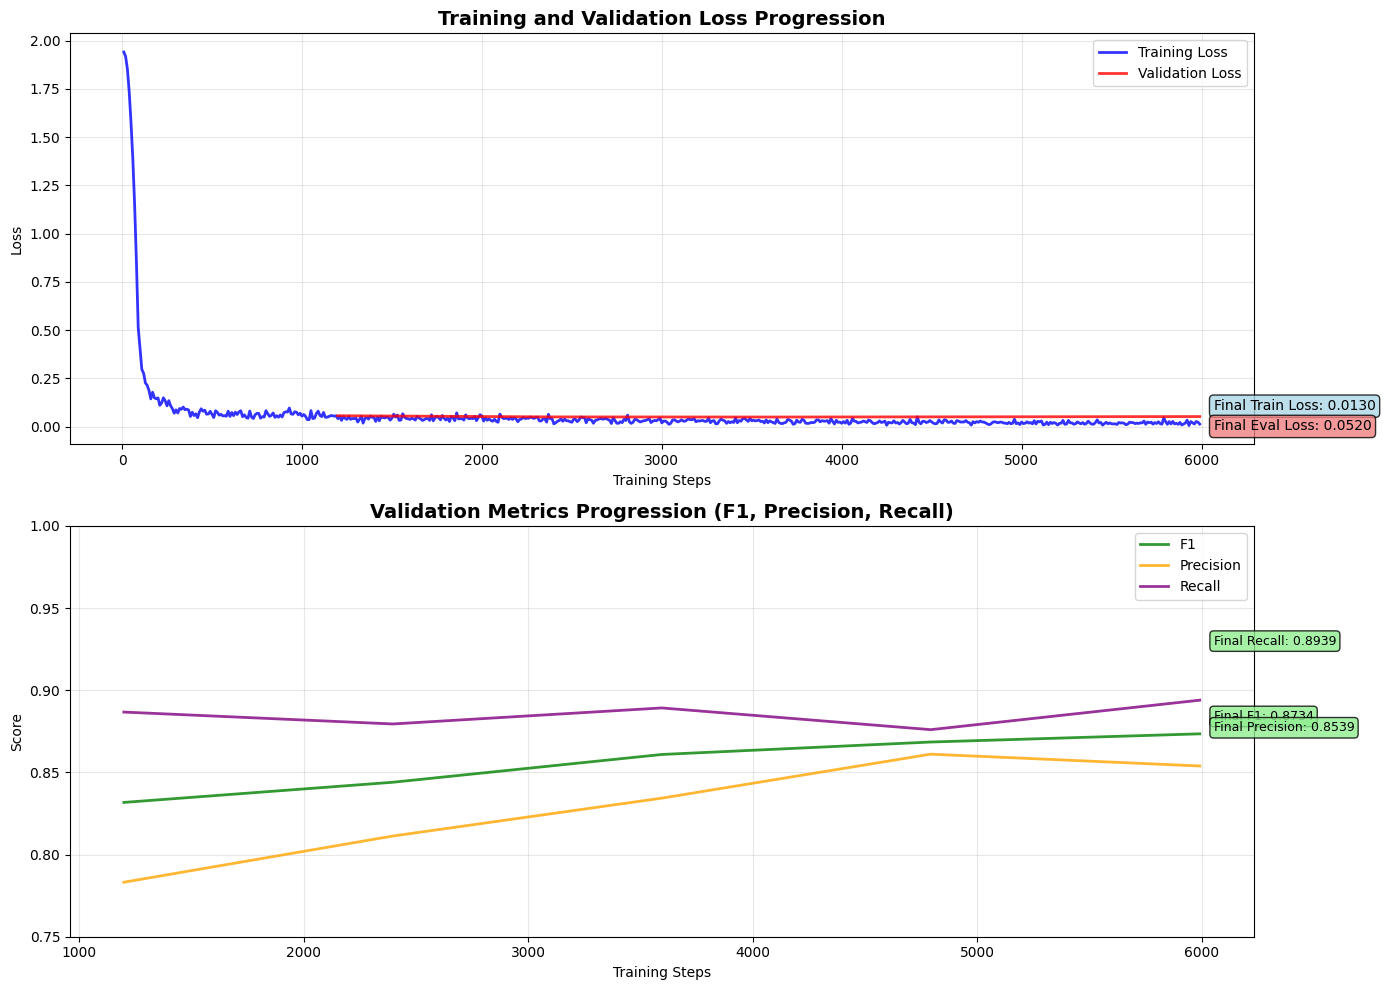
\includegraphics[width=\textwidth]{imgs/finetuning.png}
    \caption{Training and Validation Metrics of Fine-Tuned BERT NER Model}
    \label{fig:training-results}
\end{figure}


\chapter{Evaluation}
\label{ch:Evaluation}

\section{Evaluation Procedure}

To compare the performance of the different extractors, we defined a unified evaluation pipeline:

\begin{itemize}
  \item We load the cleaned dataset \texttt{full\_data\_clean.csv} and apply a 80/20 split into training and testing data.
  \item We evaluate each model configuration stored in \texttt{MODEL\_CONFIGS}. Each configuration specifies which extractor to use for each of the three entity types: \texttt{persons}, \texttt{organizations}, and \texttt{locations}.
  \item For each configuration:
  \begin{itemize}
    \item A \texttt{MultiEntityExtractor} is instantiated and fitted on the training data.
    \item Predictions are computed on the test set.
    \item The true and predicted entities are stored in a dataframe for evaluation.
    \item Entity-level evaluation metrics (precision, recall, F1) are computed and saved for each entity type.
    \item Runtime metrics such as training time, inference time, and total processing time are also recorded.
  \end{itemize}
  \item This full procedure is repeated 5 times to account for variability due to data splits.
  \item All results, including individual prediction files and metadata, are saved to disk for later analysis.
\end{itemize}

This procedure enables a fair comparison across all implemented extractors and highlights differences in computational efficiency, robustness, and prediction accuracy per entity type. Note, that the LLM method was removed as it's inference times were too slow to reasonably consider for further steps. 

\section{Results}
\section{Evaluation Procedure and Results}

\subsection{Evaluation Procedure}

To assess the effectiveness of each implemented entity extraction method, we design a consistent evaluation pipeline implemented in \texttt{05\_evaluation\_multi\_pass.py}. The evaluation involves computing standard classification metrics—\textit{precision}, \textit{recall}, \textit{F1-score}, \textit{accuracy}, and \textit{Jaccard index}—on a held-out set of human-annotated text snippets. These metrics are computed independently for each target entity type: \textit{persons}, \textit{organizations}, and \textit{locations}. Each model is evaluated in isolation and the predictions are compared against ground truth annotations.

\subsection{Performance across Metrics for Each Entity Type}

\begin{figure}[htb]
    \centering
    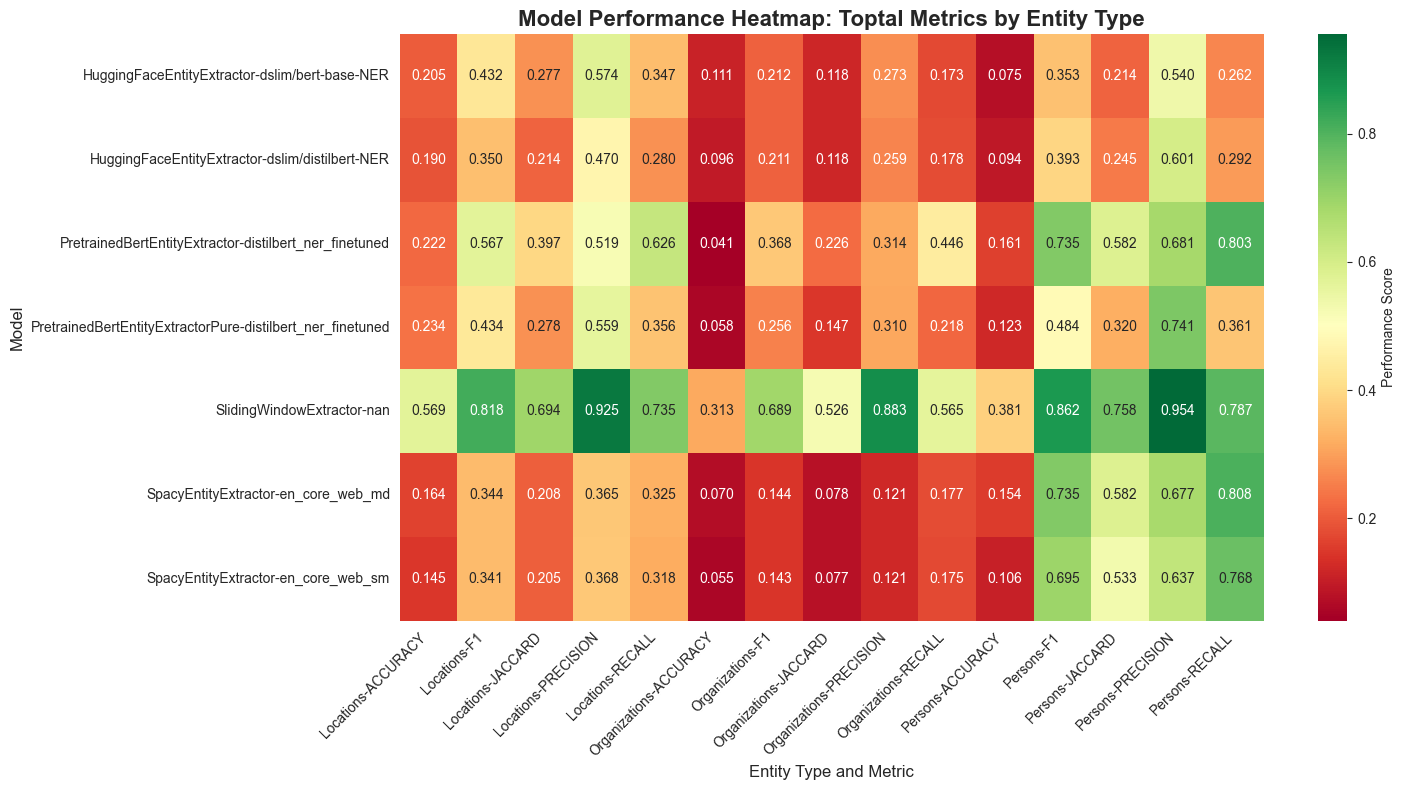
\includegraphics[width=\textwidth]{imgs/heatmap.png}
    \caption{Model performance heatmap across metrics and entity types}
    \label{fig:heatmap}
\end{figure}

Figure~\ref{fig:heatmap} and Figure~\ref{fig:ranking_f1} summarize how the different extractors perform across entity types. Surprisingly, the naive rule-based \texttt{SlidingWindowExtractor}, which simply applies lexical matching over a moving context window, outperforms all transformer-based and statistical models in nearly every metric and across all entity types. Its high recall and competitive precision contribute to top scores in F1 and Jaccard metrics. Although counterintuitive, this result is a strong reminder that domain-specific structure and simple heuristics can, in some contexts, outperform general-purpose deep learning models.

Among the non-naive models, SpaCy's large English model (\texttt{en\_core\_web\_lg}) is the best-performing statistical model, especially for \textit{person} entity extraction, followed closely by the medium and small variants. Transformer-based extractors from HuggingFace generally perform worse in absolute terms, particularly those fine-tuned on pseudo-labelled in-domain data. Their F1 scores lag behind both SpaCy and rule-based baselines, despite their theoretical advantages. One notable exception is the \texttt{dbmdz/bert-large-cased-conll03} model, which shows comparatively strong performance for \textit{locations}.

Interestingly, the models we fine-tuned ourselves (e.g., \texttt{PretrainedBERTEntityExtractor}) perform considerably worse than the out-of-the-box options. This appears to be due to limitations in the pseudo-labelling process, which introduced noise and resulted in overfitting on the dominant non-entity classes, even with mitigation strategies like hinge loss and dropout. Their F1 scores hover below 0.2 for all entity types, significantly trailing all other approaches.

\subsection{F1 Score by Entity Type}

\begin{figure}[htb]
    \centering
    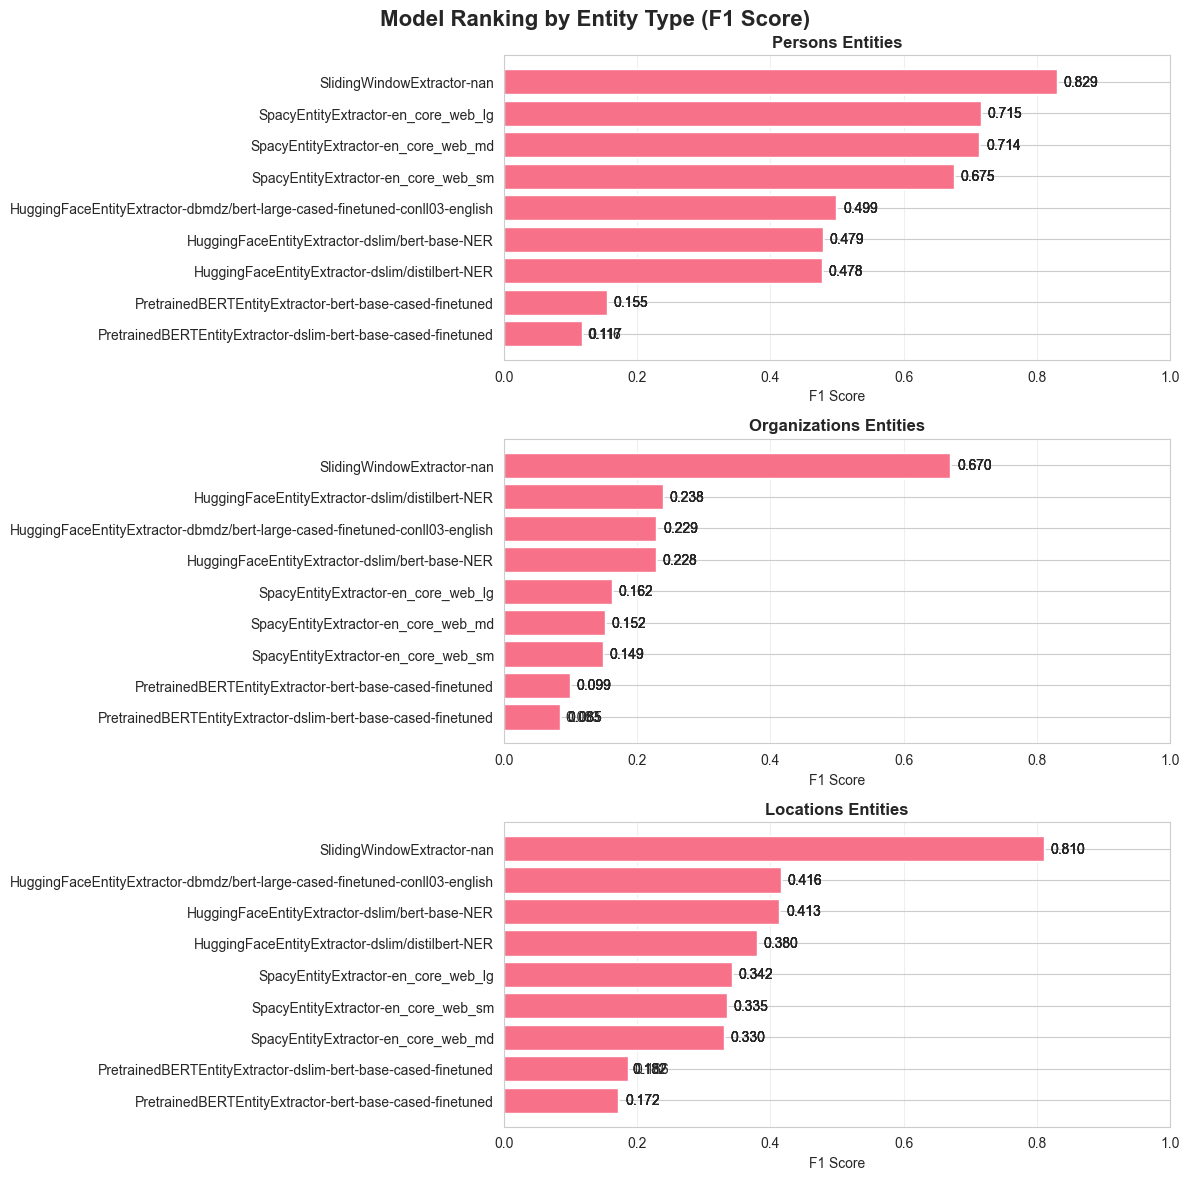
\includegraphics[width=\textwidth]{imgs/entity_type.png}
    \caption{Model ranking by entity type (F1 Score)}
    \label{fig:ranking_f1}
\end{figure}


When focusing solely on F1 scores (see Figure~\ref{fig:ranking_f1}), the superiority of the naive approach becomes even clearer. For each entity type—\textit{persons}, \textit{organizations}, and \textit{locations}—it maintains a clear lead. SpaCy’s \texttt{en\_core\_web\_lg} ranks second for person entities, offering a strong balance of coverage and specificity. For organizations, HuggingFace’s \texttt{distilbert-NER} achieves the second-highest F1 score, while for locations, the pretrained \texttt{bert-large-conll03} extractor is most competitive after the rule-based method.

Overall, F1 scores are generally highest for \textit{persons}, with precision significantly exceeding recall in most models. \textit{Organizations} and especially \textit{locations} are more challenging, often due to overlapping surface forms and more context-dependent recognition patterns. The large variance in performance between entity types also reinforces the need to evaluate NER models beyond global averages.

\subsection{Accuracy vs. Efficiency Trade-off}

Model performance cannot be evaluated on accuracy alone—especially when considering deployment in real-time or large-scale applications. Figure~\ref{fig:tradeoff} visualizes the trade-off between mean F1 score and average inference time per token. The naive extractor, while highly accurate, is clearly the slowest. This is due to its token-by-token sliding mechanism which becomes computationally expensive for longer texts.

In contrast, transformer models—especially the HuggingFace variants—are markedly more efficient. Their inference time per token is significantly lower, and they cluster tightly in the bottom-left quadrant of the plot. However, their reduced accuracy limits their applicability for precision-critical domains. SpaCy models emerge as a pragmatic compromise. They are reasonably efficient while still retaining acceptable performance, particularly for extracting person entities. These findings suggest that if latency is a strict constraint, SpaCy models may provide the best balance, while in settings where accuracy is paramount and latency is secondary, the rule-based method may remain surprisingly competitive.




\begin{figure}[htb]
    \centering
    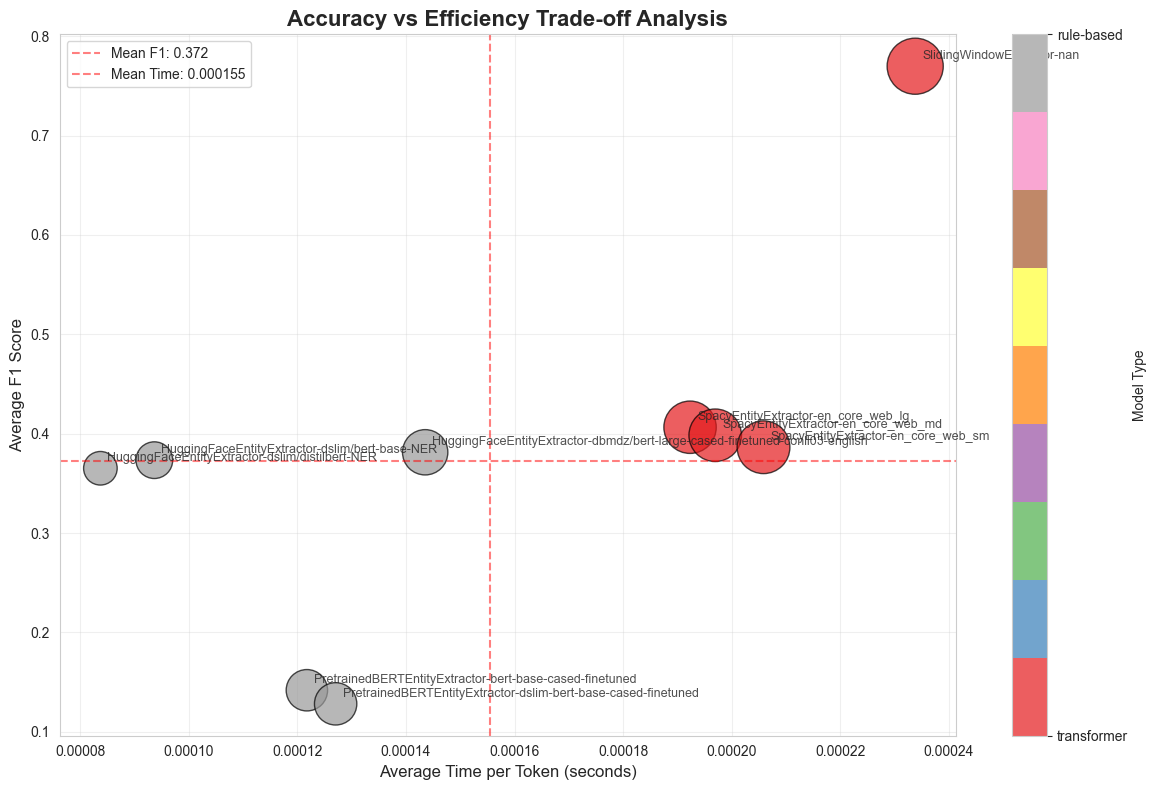
\includegraphics[width=\textwidth]{imgs/tradeoff.png}
    \caption{Trade-off between accuracy (F1) and efficiency (inference time per token)}
    \label{fig:tradeoff}
\end{figure}


\chapter{Conclusions}
\label{ch:Conclusion}

\section{Model Selection}

Based on the empirical evaluation, the \texttt{distilbert-NER} model from HuggingFace was ultimately selected for deployment. While it does not achieve top scores in terms of absolute accuracy—being outperformed by simpler rule-based and SpaCy models in several metrics—it offers significant advantages in terms of inference speed and generalizability to unseen data. Its transformer-based architecture allows it to handle complex linguistic variations and recognize entities beyond the scope of the training dataset, which is essential in a real-world, evolving environment.

The model is persisted and made accessible via environment-based configuration paths, as implemented in \texttt{07\_train\_and\_save.py}. For deployment, the model is encapsulated in a lightweight RESTful API built with FastAPI and containerized using Docker for reproducibility and portability.

Due to GPU deployment issues encountered in the production environment, the model currently runs on CPU. This constraint significantly impacts inference latency, reducing the benefits of the model’s inherent efficiency. Addressing the hardware configuration and re-enabling GPU acceleration remains a high-priority future task.

\section{Model Improvement Strategies}

The relatively poor performance of the fine-tuned models—despite architectural advantages—highlighted several opportunities for improvement:

First, the quality of the fine-tuning dataset plays a crucial role. The current dataset was generated via pseudo-labelling using GPT-4o-mini, which introduced noise and inconsistencies. Enhancing the labelling process, either through manual verification or more reliable model-generated annotations, is likely to improve downstream model performance.

Second, increasing the number of training examples would help the model generalize better and reduce overfitting to noisy or non-entity-dominated sequences. The current dataset is limited in size and may not reflect the full linguistic variability found in the target domain.

Third, the model suffers from class imbalance, particularly due to the dominance of non-entity tokens. This skew impacts both loss optimization and metric performance. Applying over-sampling of underrepresented classes or under-sampling of the majority class—combined with loss weighting or margin-based objectives like hinge loss—could yield more balanced learning.

Future work could also explore alternative model architectures or multi-task training setups that incorporate syntactic or contextual cues to further boost robustness and accuracy.
